

\tikzset{every picture/.style={line width=0.75pt}} %set default line width to 0.75pt        

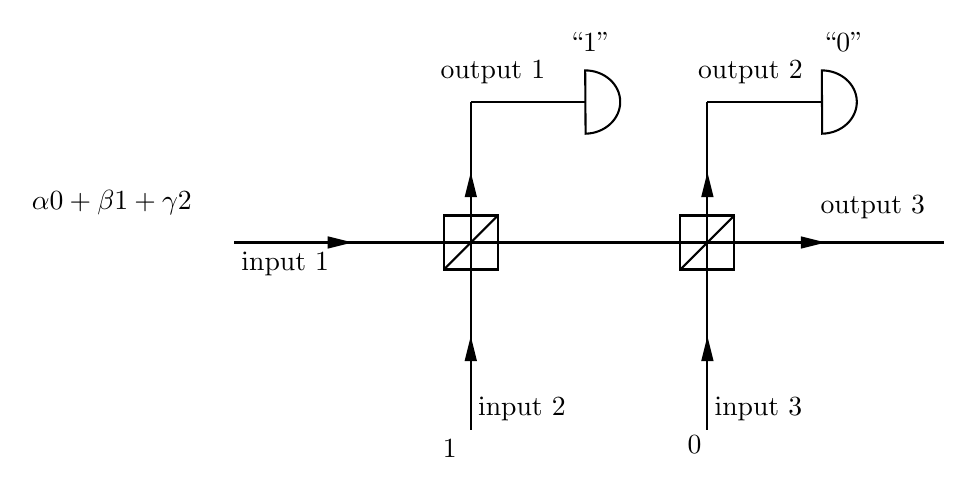
\begin{tikzpicture}[x=0.75pt,y=0.75pt,yscale=-1,xscale=1]
%uncomment if require: \path (0,300); %set diagram left start at 0, and has height of 300

%Shape: Square [id:dp5812640844481787] 
\draw   (206,108) -- (232,108) -- (232,134) -- (206,134) -- cycle ;
%Straight Lines [id:da23406010312221892] 
\draw    (206,134) -- (232,108) ;

%Straight Lines [id:da12470247976338489] 
\draw    (105,121) -- (219,121) ;
\draw [shift={(162,121)}, rotate = 180] [fill={rgb, 255:red, 0; green, 0; blue, 0 }  ][line width=0.08]  [draw opacity=0] (12,-3) -- (0,0) -- (12,3) -- cycle    ;
%Straight Lines [id:da8231064877854108] 
\draw    (219,121) -- (333,121) ;
%Straight Lines [id:da03344738041998285] 
\draw    (219,121) -- (219,211.33) ;
\draw [shift={(219,166.17)}, rotate = 90] [fill={rgb, 255:red, 0; green, 0; blue, 0 }  ][line width=0.08]  [draw opacity=0] (12,-3) -- (0,0) -- (12,3) -- cycle    ;
%Straight Lines [id:da3041250062025471] 
\draw    (219,53.33) -- (219,121) ;
\draw [shift={(219,87.17)}, rotate = 90] [fill={rgb, 255:red, 0; green, 0; blue, 0 }  ][line width=0.08]  [draw opacity=0] (12,-3) -- (0,0) -- (12,3) -- cycle    ;
%Shape: Square [id:dp9371797224374869] 
\draw   (320,108) -- (346,108) -- (346,134) -- (320,134) -- cycle ;
%Straight Lines [id:da05948010816759908] 
\draw    (320,134) -- (346,108) ;

%Straight Lines [id:da4093214516440322] 
\draw    (333,121) -- (447,121) ;
\draw [shift={(390,121)}, rotate = 180] [fill={rgb, 255:red, 0; green, 0; blue, 0 }  ][line width=0.08]  [draw opacity=0] (12,-3) -- (0,0) -- (12,3) -- cycle    ;
%Straight Lines [id:da3614482552806686] 
\draw    (333,121) -- (333,211.33) ;
\draw [shift={(333,166.17)}, rotate = 90] [fill={rgb, 255:red, 0; green, 0; blue, 0 }  ][line width=0.08]  [draw opacity=0] (12,-3) -- (0,0) -- (12,3) -- cycle    ;
%Straight Lines [id:da7606039605325201] 
\draw    (333,53.33) -- (333,121) ;
\draw [shift={(333,87.17)}, rotate = 90] [fill={rgb, 255:red, 0; green, 0; blue, 0 }  ][line width=0.08]  [draw opacity=0] (12,-3) -- (0,0) -- (12,3) -- cycle    ;
%Straight Lines [id:da4133297014948891] 
\draw    (219,53.33) -- (274,53.33) ;
%Straight Lines [id:da6242316516385615] 
\draw    (333,53.33) -- (388,53.33) ;
%Shape: Chord [id:dp8695097730726187] 
\draw   (274.11,38.08) .. controls (283.31,38.1) and (290.82,44.7) .. (290.98,53) .. controls (291.14,61.42) and (283.68,68.4) .. (274.3,68.58) -- cycle ;
%Shape: Chord [id:dp8381933152038832] 
\draw   (388.11,38.08) .. controls (397.31,38.1) and (404.82,44.7) .. (404.98,53) .. controls (405.14,61.42) and (397.68,68.4) .. (388.3,68.58) -- cycle ;

% Text Node
\draw (6,94.4) node [anchor=north west][inner sep=0.75pt]    {$\alpha \ket{0} +\beta \ket{1} +\gamma \ket{2}$};
% Text Node
\draw (204,214.4) node [anchor=north west][inner sep=0.75pt]    {$\ket{1}$};
% Text Node
\draw (322,212.4) node [anchor=north west][inner sep=0.75pt]    {$\ket{0}$};
% Text Node
\draw (265,18) node [anchor=north west][inner sep=0.75pt]   [align=left] {``1''};
% Text Node
\draw (387,18) node [anchor=north west][inner sep=0.75pt]   [align=left] {``0''};
% Text Node
\draw (107,124) node [anchor=north west][inner sep=0.75pt]   [align=left] {input 1};
% Text Node
\draw (221,208.33) node [anchor=south west] [inner sep=0.75pt]   [align=left] {input 2};
% Text Node
\draw (335,208.33) node [anchor=south west] [inner sep=0.75pt]   [align=left] {input 3};
% Text Node
\draw (203,32) node [anchor=north west][inner sep=0.75pt]   [align=left] {output 1};
% Text Node
\draw (327,32) node [anchor=north west][inner sep=0.75pt]   [align=left] {output 2};
% Text Node
\draw (386,97) node [anchor=north west][inner sep=0.75pt]   [align=left] {output 3};


\end{tikzpicture}
